\documentclass[10pt,journal,compsoc]{IEEEtran}

\usepackage{ctex}
\usepackage[dvipsnames]{xcolor}
\usepackage{times}
\usepackage{epsfig}
\usepackage{graphicx}
\usepackage{amsmath}
\usepackage{amssymb}
\usepackage{hyperref}
\usepackage{enumerate}
\usepackage{enumitem}
\usepackage{caption}
\usepackage{color}
\usepackage{comment}
\usepackage{url}
\usepackage{xcolor}
\usepackage{tabu}
\usepackage{booktabs}
\usepackage{makecell}
\usepackage{wrapfig}
\usepackage{breakcites}
\usepackage{subfig}
\usepackage{ragged2e}
\usepackage{stfloats}
\usepackage{xcolor}
\usepackage[export]{adjustbox}
\usepackage{indentfirst}
\setlength{\parindent}{2em} 

\usepackage{bm}
\usepackage{textcomp} %命令\textacutedbl的包,二阶导符号

\makeatletter
\makeatother
\let\algorithm\relax
\let\endalgorithm\relax
\usepackage[linesnumbered,ruled,vlined]{algorithm2e}%[ruled,vlined]{
\usepackage{algpseudocode}
\renewcommand{\algorithmicrequire}{\textbf{Input:}}
\renewcommand{\algorithmicensure}{\textbf{Output:}}

\usepackage{tikz}
\usetikzlibrary{backgrounds}
\usetikzlibrary{arrows,shapes}
\usetikzlibrary{tikzmark}
\usetikzlibrary{calc}

\usepackage{amsmath}
\usepackage{amsthm}
\usepackage{amssymb}
\usepackage{mathtools, nccmath}
\usepackage{wrapfig}
\usepackage{comment}

% To generate dummy text
\usepackage{blindtext}

\usepackage{graphicx}
\usepackage{xspace}

% table alignment
\usepackage{array}
\usepackage{ragged2e}
\newcolumntype{P}[1]{>{\RaggedRight\hspace{0pt}}p{#1}}
\newcolumntype{X}[1]{>{\RaggedRight\hspace*{0pt}}p{#1}}

% color box
\usepackage{tcolorbox}


% for tikz
\usepackage{tikz}
\usetikzlibrary{arrows,shapes,positioning,shadows,trees,mindmap}
\usepackage[edges]{forest}
\usetikzlibrary{arrows.meta}
\colorlet{linecol}{black!75}
\usepackage{xkcdcolors} % xkcd colors


% for colorful equation
\usepackage{tikz}
\usetikzlibrary{backgrounds}
\usetikzlibrary{arrows,shapes}
\usetikzlibrary{tikzmark}
\usetikzlibrary{calc}
% Commands for Highlighting text -- non tikz method
\newcommand{\highlight}[2]{\colorbox{#1!17}{$\displaystyle #2$}}
\newcommand{\highlightdark}[2]{\colorbox{#1!47}{$\displaystyle #2$}}

% my custom colors for shading
\colorlet{mhpurple}{Plum!80}


% Commands for Highlighting text -- non tikz method
\renewcommand{\highlight}[2]{\colorbox{#1!17}{#2}}
\renewcommand{\highlightdark}[2]{\colorbox{#1!47}{#2}}

% Some math definitions
\newcommand{\lap}{\mathrm{Lap}}
\newcommand{\pr}{\mathrm{Pr}}

\newcommand{\Tset}{\mathcal{T}}
\newcommand{\Dset}{\mathcal{D}}
\newcommand{\Rbound}{\widetilde{\mathcal{R}}} 

%\usepackage{algorithm}
%\usepackage[noend]{algpseudocode}

% 定义代码样式
\usepackage{listings}

\definecolor{gray}{rgb}{0.96,0.96,0.96}

\lstset{ %
  language=python,                % the language of the code
  basicstyle=\footnotesize,           % the size of the fonts that are used for the code
  numbers=left,                   % where to put the line-numbers
  columns=fixed, 
  numberstyle=\tiny\color{black},  % the style that is used for the line-numbers
  stepnumber=1,                   % the step between two line-numbers. If it's 1, each line 
                                  % will be numbered
  numbersep=1.5mm,                  % how far the line-numbers are from the code
  xleftmargin=1.3em,
  backgroundcolor=\color{gray},      % choose the background color. You must add \RequirePackage{color}
  showspaces=false,               % show spaces adding particular underscores
  showstringspaces=false,         % underline spaces within strings
  showtabs=false,                 % show tabs within strings adding particular underscores
  frame=single,,                 % adds a frame around the code
  frameround = tttt,
  framexleftmargin=3mm, 
  rulecolor=\color[RGB]{158,193,243},        % if not set, the frame-color may be changed on line-breaks within not-black text (e.g. commens (green here))
%  aboveskip=1em,
  tabsize=2,                      % sets default tabsize to 2 spaces
  captionpos=b,                   % sets the caption-position to bottom
  breaklines=true,                % sets automatic line breaking
  extendedchars=false,   
  breakatwhitespace=false,        % sets if automatic breaks should only happen at whitespace
  title=\lstname,                   % show the filename of files included with \lstinputlisting;
                                  % also try caption instead of title
  keywordstyle=\color[RGB]{0,51,179},          % keyword style
  commentstyle=\color[RGB]{140,140,140},       % comment style
  stringstyle=\color[RGB]{6,125,23},         % string literal style
  identifierstyle=\color{black},
  escapeinside={\%*}{*)},            % if you want to add LaTeX within your code
  morekeywords={*,...}               % if you want to add more keywords to the set
}

\def\Plus{\texttt{+}}

\makeatletter
\def\BState{\State\hskip-\ALG@thistlm}
\makeatother

\graphicspath{{figures/}}

% *** CITATION PACKAGES ***
%
\ifCLASSOPTIONcompsoc
  % IEEE Computer Society needs nocompress option
  % requires cite.sty v4.0 or later (November 2003)
  \usepackage[nocompress]{cite}
\else
  % normal IEEE
  \usepackage{cite}
\fi

% *** GRAPHICS RELATED PACKAGES ***
%
\ifCLASSINFOpdf

\else

\fi

\hyphenation{op-tical net-works semi-conduc-tor}


\begin{document}
\begin{sloppypar}

\title{计算机视觉作业­5:背景建模}

\author{唐麒\qquad 21120299\\qitang@bjtu.edu.cn}

\IEEEtitleabstractindextext{
\begin{abstract}
\justifying 在运动目标检测提取中,背景目标对于目标识别和跟踪至关重要。图像变化的原因一般分成相机运动和相机固定。前者一般用光流法,后者一般用背景建模法。基于高斯混合模型的背景建模适合于在相机固定的情况下,从图像序列中分离出背景和前景。其在物体具有重复性运动的情况下鲁棒性较好,比如微风树叶抖动。本文将对基于高斯混合模型的背景建模方法进行介绍,其效果及实时性分析在实验部分给出。

\end{abstract}

\begin{IEEEkeywords}
计算机视觉、背景建模、高斯混合模型
\end{IEEEkeywords}}


% make the title area
\maketitle

\IEEEraisesectionheading{\section{简介}
\label{sec:introduction}}

在计算机视觉众多的技术领域中,目标检测(Object Detection)也是一项非常基础的任务,图像分割、物体追踪、关键点检测等通常都要依赖于目标检测。在目标检测时,由于每张图像中物体的数量、大小及姿态各有不同,也就是非结构化的输出,这是与图像分类非常不同的一点,并且物体时常会有遮挡截断,所以物体检测技术也极富挑战性,从诞生以来始终是研究学者最为关注的焦点领域之一。

在计算机视觉中,图像分类、目标检测和图像分割都属于最基础、也是目前发展最为迅速的3个领域,如图 \ref{fig:cv_task} 所示,这几个任务之间的区别为:

\begin{itemize}
	\item 图像分类:输入图像往往仅包含一个物体,目的是判断每张图像是什么物体,是图像级别的任务,相对简单,发展也最快。
	\item 目标检测:输入图像中往往有很多物体,目的是判断出物体出现的位置与类别,是计算机视觉中非常核心的一个任务。
	\item 图像分割:输入与物体检测类似,但是要判断出每一个像素属于哪一个类别,属于像素级的分类。图像分割与物体检测任务之间有很多联系,模型也可以相互借鉴。
\end{itemize}

在利用深度学习做物体检测之前,传统算法对于目标检测通常分为3个阶段:区域选取、特征提取和体征分类。首先选取图像中可能出现物体的位置,由于物体位置、大小都不固定,因此传统算法通常使用滑动窗口(Sliding Windows)算法,但这种算法会存在大量的冗余框,并且计算复杂度高。在得到物体位置后,通常使用人工精心设计的提取器进行特征提取,如 SIFT 和 HOG 等。由于提取器包含的参数较少,并且人工设计的鲁棒性较低,因此特征提取的质量并不高。最后,对上一步得到的特征进行分类,通常使用如SVM、AdaBoost的分类器。

\begin{figure}[!ht]
  \centering
  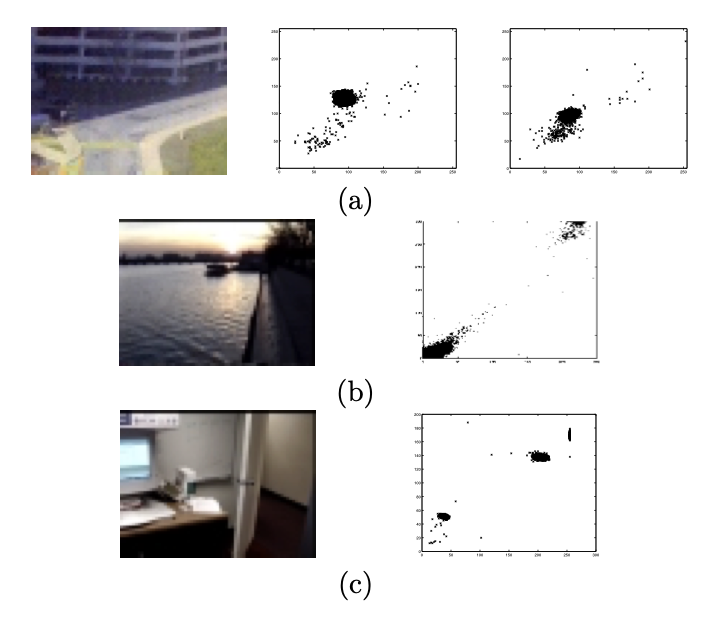
\includegraphics[width=\linewidth]{fig1}
  \caption{计算机视觉中的图像分类、目标检测和图像分割任务示意图}
  \label{fig:cv_task}
  \vspace{-0.5cm}
\end{figure}

基于深度学习的目标检测方法逐渐使目标检测进入到快速发展的阶段,比较流行的算法可以分为两类,一类是基于 Region Proposal 的R-CNN系算法(RCNN、SPPNet、FasterRCNN、Pyramid NetWorks等),它们是two-stage的,需要先算法产生目标候选框,也就是目标位置,然后再对候选框做分类与回归。而另一类是 Yolo,SSD 这类 one-stage 算法,其仅仅使用一个卷积神经网络直接预测不同目标的类别与位置。第一类方法是准确度高一些,但是速度慢,但是第二类算法是速度快,但是准确性要低一些。

本文分别利用传统的基于滑窗的目标检测算法(即机器学习方法)实现静态场景下的侧视车辆检测和基于深度学习的目标检测模型对口罩进行检测。本文剩余部分将对传统目标检测放法的原理和采用的深度学习模型的架构、实现及实验进行介绍,所有实验涉及的方法、函数实现均基于 Python 语言,其中深度学习模型的实现及训练等采用了开源深度学习框架 PyTorch。
\section{方法} 
\label{sec:proposed}

这一章节将对统计方法的纹理分析和基于聚类技术的纹理分割进行介绍,其中本文对统计方法的纹理分析采用了灰度共生矩阵和 Gabor 滤波器两种纹理特征表示方法,其对分割结果将在实验部分给出。

\subsection{纹理表示}

\subsubsection{灰度共生矩阵}

灰度共生矩阵(GLCM, Gray Level Coocurrence Matrices)是描述具有某种空间位置关系两个像素灰度的联合分布概率,不仅反映灰度的分布特性,也反映具有同样灰度或相近灰度的像素之间的位置分布特性,是有关图象灰度变化的二阶统计特征。这是由于纹理是由灰度分布在空间位置上反复出现而形成的,因而在图像空间中相隔某距离的两像素之间会存在一定的灰度关系,即图像中灰度的空间相关特性。灰度共生矩阵描述的从来不是单个像素,而是成对的像素之间的关系,对应的,灰度直方图则可以看做是对单个像素的统计与描述,并不涉及灰度间的关联关系。灰度共生矩阵能反映图像灰度关于方向、相邻间隔、变化幅度等综合信息,它是分析图像的局部模式和它们排列规则的基础。其计算公式定义为:

\begin{equation}
\begin{gathered}
P(i, j \mid \Delta x, \Delta y)=W \cdot Q(i, j \mid \Delta x, \Delta y) \\
W=\frac{1}{(M-\Delta x)(N-\Delta y)}, Q(i, j \mid \Delta x, \Delta y)=\sum_{n=1}^{N-\Delta y} \sum_{m=1}^{M-\Delta x} A \\
A=\left\{\begin{array}{cc}
1 \quad \text { if } \quad f(m, n)=i \text { and } f(m+\Delta x, y+\Delta y)=j \\
0 \text { else }
\end{array}\right.
\end{gathered}
\vspace{0.5cm}
\end{equation}

其中,$P(i,j)$ 为灰度共生矩阵中的元素,表示对于一个有着 $G$ 个灰度级、大小为 $M \times N$的图像而言,沿着图像的某一方向移动距离 $d$,像素的灰度级从 $i$ 变为 $j$ 的概率,$P(i, j \mid \Delta x, \Delta y)$ 也可以用符号 $P(i, j \mid d, \theta)$ 来表示;$f(m,n)$ 表示图像中坐标为 $(m,n)$ 的像素的灰度值。

如图 \ref{fig:glcm_figure} 所示,$x$ 方向是图像的列,$y$ 方向是图像的行,$f(x, y) = i$,为坐标 $(x, y)$ 处的灰度值,灰度共生矩阵需要统计的是距离 $(dx, dy)$ 处 $f(x + dx, y + dy) = j$ 的频数(概率),由于 $(dx, dy)$ 的选择不同,则会导致角度的不同,通常选择 $0°$、$45°$、$90°$ 和 $135°$。

\begin{figure}[!htbp]
	\centering
	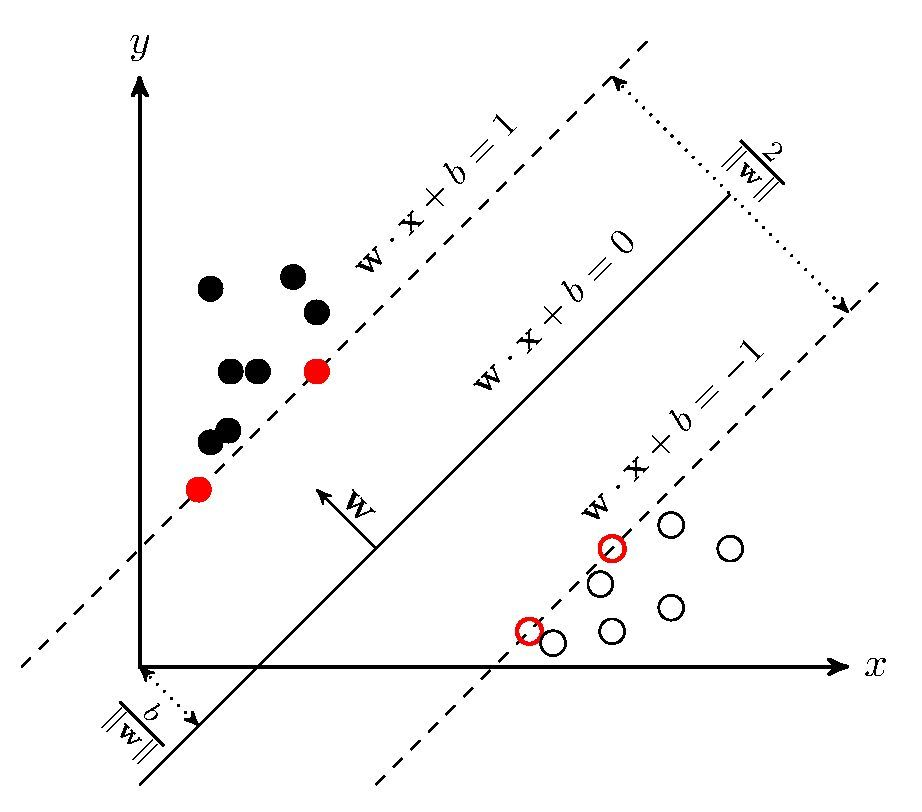
\includegraphics[width=\linewidth]{fig2}
	\caption{灰度共生矩阵的几何表示}
	\label{fig:glcm_figure}
	 \vspace{-0.5cm}
\end{figure}


灰度共生矩阵的计算量是由图像的灰度级和图像的大小共同决定的。例如,假定图像 $I$ 有 $L$ 个灰度级,其大小为 $R \times C$,则运算量大约为 $L^2 \times R \times C$。实际生活中,$L$一般为 $256$, 若令 $R=512, C=512$,则至少要 $1.7 \times 10^{10}$ 次运算,约需耗费30分钟,这显然不太切合实际的。因此在计算灰度共生矩阵时,在不影响纹理特征的前提下往往先对灰度图像的灰度值进行量化,压缩到一个较小的范围,一般取16级。代码实现如下:

\vspace{0.3cm}
\lstinputlisting[language=Python,firstline=35,lastline=41]{main.py}

除此之外,通过直方图均衡化对图像进行预处理也是计算灰度共生矩阵的常用技巧,从而可以消除绝对灰度值的影响。通常,更多地是使用各向同性的灰度共生矩阵来提取具有旋转不变性的纹理特征,即分别计算 $0°$、$45°$、$90°$ 和 $135°$ 四个方向的灰度共生矩阵,如图 \ref{fig:glcm_sample} 所示,然后求均值得到各向同性的灰度共生矩阵。

\begin{figure}[!htbp]
	\centering
	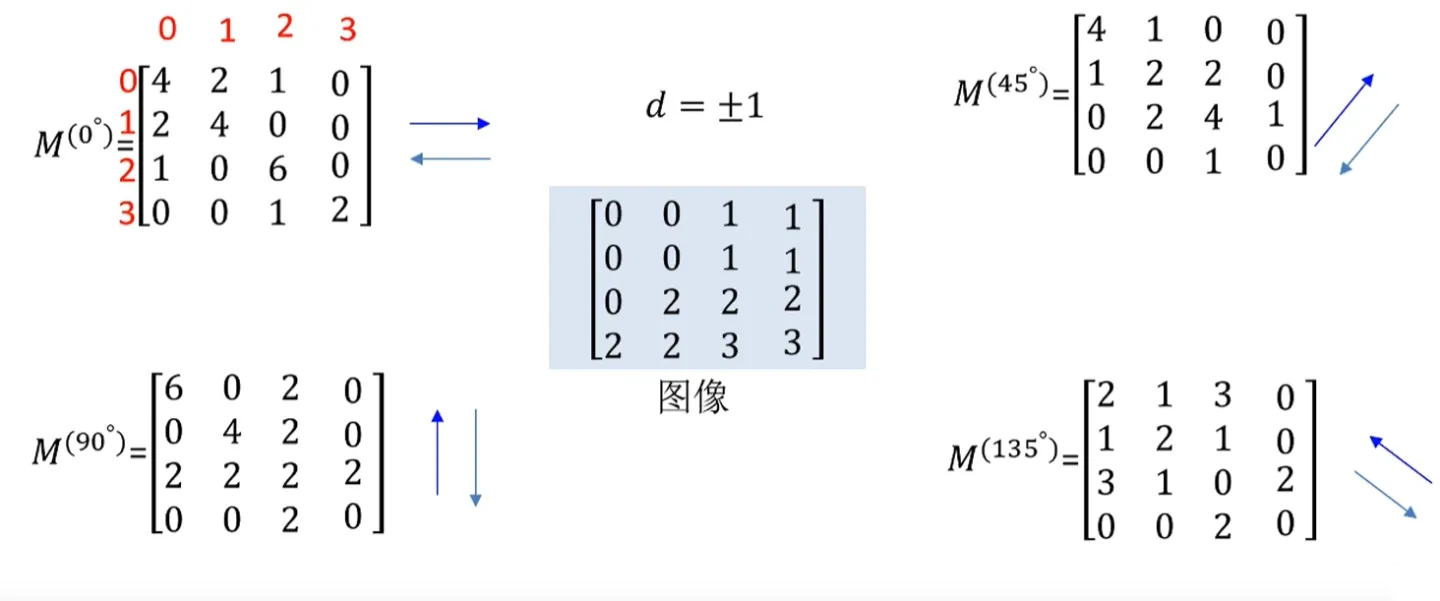
\includegraphics[width=\linewidth]{fig3}
	\caption{简单的图像矩阵及其灰度共生矩阵的示例}
	\label{fig:glcm_sample}
%	 \vspace{-0.5cm}
\end{figure}

统计方法的纹理分析都是通过统计向量(特征向量)来描述区域中的纹理,即在一个局部窗口中计算局部的纹理表征,然后在图像中滑动窗口,最终获得整个图像的纹理表征。灰度共生矩阵也是在这样一个 $w \times w$ 大小的滑动窗口中进行计算的。对于有 $G$ 个灰度级的图像而言,其灰度共生矩阵的维度为 $G \times G$。以图 \ref{fig:glcm_sample} 为例,灰度共生矩阵的计算过程如下:

\begin{enumerate}
	\item 如图 \ref{fig:glcm_sample} 所示,图像的灰度级为4,因此首先创建一个大小为 $4 \times 4$ 的空灰度共生矩阵;
	\item 分别按照 $(d = 1,θ = 0°)$ 、 $(d = 1,θ = 45°)$ 、 $(d = 1,θ = 90°)$ 和 $(d = 1,θ = 135°)$ 进行计算;
	\item 以 $(d = 1,θ = 0°)$ 为例,如第一个值,代表的是图像中灰度值为0,且其水平方向上距离一个像素的点灰度值也为0,即灰度值对 $(0, 0)$ 出现的次数;
	\item 滑动窗口遍历整个图像,并求均值即可完成灰度共生矩阵的计算。
\end{enumerate}

代码实现如下\footnote{由于篇幅原因,部分中间过程代码在此省略}:
\vspace{0.3cm}
\lstinputlisting[language=Python,firstline=118,lastline=135]{main.py}

灰度共生矩阵主要用于纹理特征的提取,但是,一般不直接采用灰度共生矩阵来进行对纹理的统计特性进行度量,而是进一步基于灰度共生矩阵构建统计量。Haralick 提出了14种基于灰度共生矩阵计算出来的统计量,即能量、熵、对比度、均匀性、相关性、方差、和平均、和方差、和熵、差方差、差平均、差熵、相关信息测度以及最大相关系数\footnote{相关统计量的计算方法将在附录 A 给出}。这些特征彼此之间具有较强的相关性,一般采用对比度、角度方向二阶矩、熵和平均值来描述纹理的特性。本文采用了如表 \ref{tab:measurement} 所示的统计量,在将统计量可视化的基础上针对不同的图像进行选择,尽可能建立最有助于纹理分割的纹理特征表示。部分代码实现如下\footnote{完整代码见附录 B}。

在获得基于灰度共生矩阵的统计量后,对其进行均值滤波和标准化处理可以获得更好的分割效果。

\vspace{0.3cm}
\lstinputlisting[language=Python,firstline=4,lastline=45]{glcm_features.py}

\subsubsection{Gabor 滤波器}

对于纹理分析而言,采用 Gabor 滤波具有较好的时-频局部话特性,它能够同时表示和捕捉二维信号在空间位置、空间频率、方向选择性和相位、频率带宽等方面的信息。用 Gabor 滤波器对图像信号滤波,相当于将其按不同方向、频段进行分解,如果计算经不同方向、频段滤波后的纹理特征,这些特征将具有明显的差异,根据这些差异就可以区分不同的纹理。在计算机视觉和图像处理中,多通道 Gabor 方法被认为是一种非常有用的工具,特别是在纹理分析方面。自从一维 Gabor 函数提出之后,很多学者对 Gabor 分析方法进行了研究,研究表明在哺乳类生物视觉系统中,特别是涉及到纹理方面,Gabor 线性空间滤波器有着非常重要的作用。本文采用的基于 Gabor 滤波器的纹理分析方法\footnote{本方法利用网络资源进行实现,由于篇幅原因其实现不再具体展示}如图 \ref{fig:gabor} 所示。

\begin{figure}[!htbp]
	\centering
	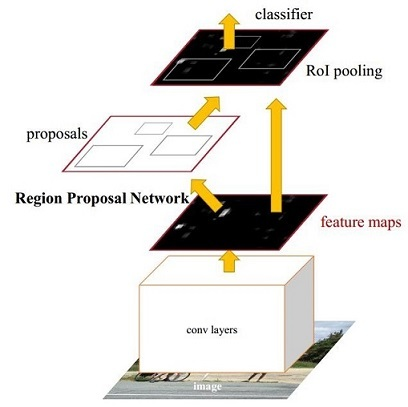
\includegraphics[width=\linewidth]{fig4}
	\caption{基于 Gabor 滤波器的纹理分析及纹理分割算法流程图}
	\label{fig:gabor}
%	 \vspace{-0.5cm}
\end{figure}

Gabor 滤波的方法实际上是多分辨率分解的过程,该方法类似小分析方法。用 Gabor 滤波器进行纹理分析有几个步骤:

\begin{enumerate}
	\item 设计一个对应于不同空间频率和方向的滤波器组;
	\item 把原图像分解为多个滤波图像;
	\item 利用 Gabor 能量特征从滤波图像中提取纹理特征;
	\item 在特征空间中聚类,生成分割图像。
\end{enumerate}

在滤波图像的基础上提取纹理特征,生成特征图像,相同特征区域中的像素具有相同的纹理特性,在特征空间中它们彼此靠近,无监督纹理分割方法即将图像像素聚类到几个簇中,并表现出缘由图像纹理区域,然后给每个簇定义新的标签实现纹理图像分割的目的。一个好的“分类器”在特征空间要实现类内距离尽量小,而类间距离尽量大。下一小节将对基于聚类技术的纹理分割进行介绍。

\subsection{纹理分割}

纹理分割本质上是一个图像分割问题,即采用聚类的方法对图像进行分割,而聚类的特征空间则是由图像的纹理特征构建的。常用的聚类方法,包括 K-Means、Mean-Shift 和 DBScan 等。相较于后者而言,K-Means 更适合本文的实验数据且收敛速度更快,因此,本文将主要对 K-Means 算法进行介绍。 K-Means 算法伪代码如下:
 
 \begin{algorithm}
        \caption{K-Means}
        \LinesNumbered
        \KwIn{输入样本集$D$ = \{$x_1,x_2,\cdots,x_N$\},分簇数$K=n$,最大迭代次数为$M$,从分簇样本中随机选取$n$点\{$u_1$,$u_2,\cdots,u_n$\}作为初始质心}
        \KwOut{输出各样本所在簇\{$C_1$,$C_2$,$\cdots$,$C_n$\}}
        
        \For(\tcp*[f]{$m$表示迭代次数}){$m = 1 \to M$} 
        {
        $C_1 \Leftarrow \emptyset, C_2 \Leftarrow \emptyset,\cdots,  C_n \Leftarrow \emptyset$\tcp*[f]{初始化各簇}
        
            \For(\tcp*[f]{$i$表示样本集编号}){$i = 1,2,...,N$ }     
            {
              $d_{i1} \Leftarrow {\Vert x_i-u_1 \Vert}^2$, $d_{i2} \Leftarrow {\Vert x_i-u_2 \Vert}^2$, $\cdots$, $d_{in} \Leftarrow {\Vert x_i-u_n \Vert}^2$ \tcp*[f]{计算$x_i$到各质心的欧式距离}
              
            \If {$argmin(d_{in}) == n$}
            { $C_n \Leftarrow C_n \cup \{x_i\}$ \tcp*[f]{将$x_i$划分到相应的簇}
            }
            }
            
             $\tilde{u_1} \Leftarrow \frac{1}{\vert C_1 \vert}\sum\limits_{x \in C_1} x$, $\tilde{u_2} \Leftarrow \frac{1}{\vert C_2 \vert}\sum\limits_{x \in C_2} x$,
             $\cdots$,
             $\tilde{u_n} \Leftarrow \frac{1}{\vert C_n \vert}\sum\limits_{x \in C_n} x$
             \tcp*[f]{重新计算各簇质心}
            
            \If(\tcp*[f]{各簇质心未改变,跳出循环}){$\forall\;\tilde{u_n},\;\tilde{u_n} == u_n$}
            {\textbf{break} from line 3 %\textbf为加粗}
            \Else{
            $u_1 \Leftarrow \tilde{u_1}, u_2 \Leftarrow \tilde{u_2}, \cdots, u_n \Leftarrow \tilde{u_n}$ \tcp*[f]{更新各簇质心}
            }
            }

           \Return $C_1, C_2, \cdots, C_n$ \tcp*[f]{输出结果}
        }
                
    \end{algorithm}
    
代码实现如下\footnote{由于篇幅原因,部分中间过程代码在此省略}:
\vspace{0.3cm}
\lstinputlisting[language=Python,firstline=242,lastline=263]{main.py}

\twocolumn[{%
\renewcommand\twocolumn[1][]{#1}%
\noindent\begin{minipage}{\linewidth} 
 	\begin{center}
 	\vspace{0.3cm}
 	\captionsetup{font=small}
 	\begin{tabular}{@{}c@{}c@{}c@{}c@{}}
 	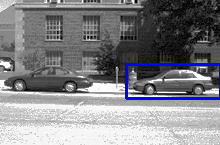
\includegraphics[width=0.24\linewidth]{fig6_a1} &
	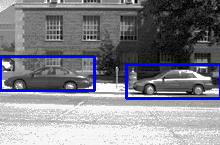
\includegraphics[width=0.24\linewidth]{fig6_b1} &
 	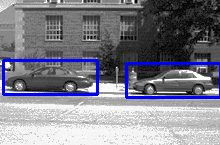
\includegraphics[width=0.24\linewidth]{fig6_c1} &
 	 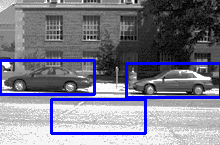
\includegraphics[width=0.24\linewidth]{fig6_d1} \vspace{-1mm}\\ 
 	 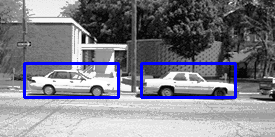
\includegraphics[width=0.24\linewidth]{fig6_a2} &
	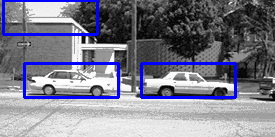
\includegraphics[width=0.24\linewidth]{fig6_b2} &
	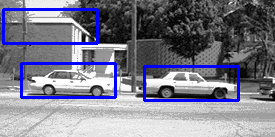
\includegraphics[width=0.24\linewidth]{fig6_c2} &
 	 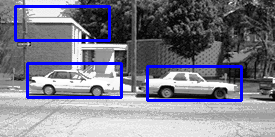
\includegraphics[width=0.24\linewidth]{fig6_d2} \vspace{-1mm}\\   
    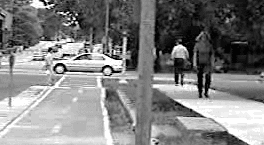
\includegraphics[width=0.24\linewidth]{fig6_a3} &
	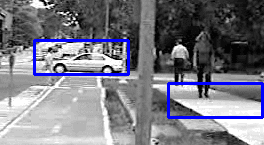
\includegraphics[width=0.24\linewidth]{fig6_b3} &
 	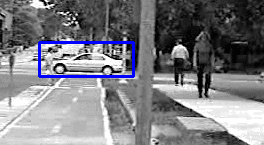
\includegraphics[width=0.24\linewidth]{fig6_c3} &
 	 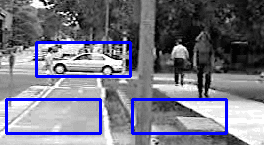
\includegraphics[width=0.24\linewidth]{fig6_d3}  \vspace{-1mm}\\
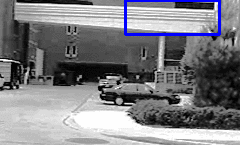
\includegraphics[width=0.24\linewidth]{fig6_a4} &
	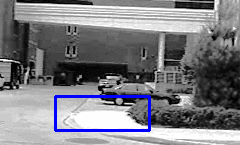
\includegraphics[width=0.24\linewidth]{fig6_b4} &
 	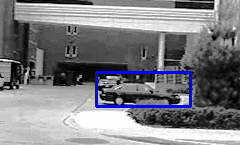
\includegraphics[width=0.24\linewidth]{fig6_c4} &
 	 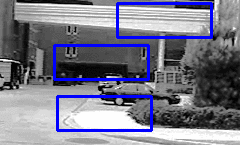
\includegraphics[width=0.24\linewidth]{fig6_d4} \vspace{-1mm}\\

    {\small (a)} &  {\small (b)}  &  {\small (c)} &  {\small (d)} \\
    \end{tabular}
	\captionof{figure}{\small 不同分类器在车辆侧视数据集上的检测结果。(a) Logistic 回归, (b) 支持向量机, (c) AdaBoost, and (d) AdaBoost$^*$.}
	\label{fig:result}
	\end{center}
	\vspace{0.5cm}
\end{minipage}
}]

\section{实验}
\label{sec:experiment}


这一章节将会利用上一章介绍的高斯混合模型的背景建模方法在视频序列图像上进行实验,并对其实现效果、实时性进行展示和分析。

\subsection{数据集}

传统的基于滑窗的目标检测算法将在静态场景下的侧视车辆数据集上进行实验,其中训练集包含 550 个正例样本和 500 个负例样本,共有 170 张测试图片。利用 sklearn 中的 train\_test\_split 方法按照 4:1 对数据集进行训练集和验证集的划分。划分好数据集后,利用 HOG 对训练集数据的图片进行特征提取并对 PCA 降维模型进行训练,将 27104 维数据降维至 300 维。

基于深度学习的口罩检测将在 Mask Wearing 数据集上进行实验,数据集包含用于训练模型的图像 468 张、用于模型验证的图像 116张和用于模型性能测试的图像 95 张。图像的标签以 xml 格式标注,标注文件中包含目标的类别(good:佩戴口罩,bad:未佩戴口 罩,none:未正确佩戴口罩)及其边界框左上角和右下角的(x,y)坐标值。

\subsection{评价指标}

选择 Recall、Precision 和 F-measure 指标对模型结果进行评测。在介绍这三个指标前需要明确四个概念:TP、FP、TN、FN。


\begin{table}[htbp]
  \centering
  \caption{分类结果混淆矩阵}
  \setlength{\tabcolsep}{7mm}{
    \begin{tabular}{c|c|c}
    \toprule
    \multirow{2}[4]{*}{真实情况} & \multicolumn{2}{c}{预测结果} \\
\cmidrule{2-3}          & 正例    & 反例 \\
    \midrule
    正例    & TP(真正例) & FN(假反例) \\
    \midrule
    反例    & FP(假正例) & TN(真反例) \\
    \bottomrule
    \end{tabular}%
  \label{tab:matrixl}}
\end{table}%


Recall、Precision 和 F-measure 相应的计算方法如下: 

\begin{equation}
\begin{aligned}
	查全率(precision) &= \frac{TP}{TP+FP}\\
	查准率(recall) &= \frac{TP}{TP+FN}
\end{aligned}
\end{equation}

查全率和查准率是一对矛盾的度量,一般来说,查准率高时,查全率往往偏低;而查全率高时,查准率往往偏低。通常只有在一些简单任务中,才可能使查全率和查准率都很高。在两者都要求高的情况下,综合衡量查全率和查准率就用 F1 值,其计算方法如下:

\begin{equation}
	F1 = \frac{2\times precision \times recall}{precision + recall}
\end{equation}

\subsection{车辆检测}

不同分类器的训练结果如表 \ref{tab:class_result} 所示,其中 AdaBoost$^*$ 表示采用参数 algorithm='SAMME.R', learning\_rate=1.0, n\_estimators=100, random\_state=0 训练得到的分类器。测试时,利用与训练图片等大的窗口大小对待检测图片进行滑窗。然后对每个窗进行分类,判断其是否为汽车。如果是汽车则将其保存为候选,最后利用所有候选带入 NMS 算法计算得到最终的检测框。由于测试集未给出标签,统计结果如表 \ref{tab:count} 所示,计算指标如表 \ref{tab:metric}所示,部分检测结果如图 \ref{fig:result} 所示。

\begin{table*}[!ht]
	\centering
	\caption{分类器训练测试结果表}
	\begin{subtable}[t]{0.495\linewidth}
	\caption{Logistic 回归}
	\begin{tabular}{c|cccc}
		\toprule
		& Precision&Recall & F1 Score &Support\\\hline
		no car&1.00&0.97&0.99&109\\
		car &0.97&1.00&0.99&101\\\hline
		accuracy&&&0.99&210\\ 
		macro average &0.99&0.99&0.99&210\\
		weighted avg&0.99&0.99&0.99&210\\
		\bottomrule
	\end{tabular}
	\end{subtable}
	\begin{subtable}[t]{0.495\linewidth}
	\caption{支持向量机}
	\begin{tabular}{c|cccc}
		\toprule
		& Precision&Recall & F1 Score &Support\\\hline
		no car&0.99&1.00&1.00&105\\
		car &1.00&0.99&1.00&105\\\hline
		accuracy&&&1.00&210\\ 
		macro average &1.00&1.00&1.00&210\\
		weighted avg&1.00&1.00&1.00&210\\
		\bottomrule
	\end{tabular}
	\end{subtable}

	\begin{subtable}[t]{0.495\linewidth}
	\caption{AdaBoost}
	\begin{tabular}{c|cccc}
		\toprule
		& Precision&Recall & F1 Score &Support\\\hline
		no car&1.00&0.96&0.98&102\\
		car &0.96&1.00&0.98&108\\\hline
		accuracy&&&0.98&210\\ 
		macro average &0.98&0.98&0.98&210\\
		weighted avg&0.98&0.98&0.98&210\\
		\bottomrule
	\end{tabular}
	\end{subtable}
	\begin{subtable}[t]{0.495\linewidth}
	\caption{AdaBoost$^*$}
		\begin{tabular}{c|cccc}
		\toprule
		& Precision&Recall & F1 Score &Support\\\hline
		no car&1.00&1.00&1.00&109\\
		car &1.00&1.00&1.00&101\\\hline
		accuracy&&&1.00&210\\ 
		macro average &1.00&1.00&1.00&210\\
		weighted avg&1.00&1.00&1.00&210\\
		\bottomrule
	\end{tabular}
	\end{subtable}
	\label{tab:class_result}
\end{table*}

\begin{table}[!ht]
\centering
\caption{不同分类器的检测结果}
\setlength{\tabcolsep}{6mm}{
\begin{tabular}{c|c|c|c}
	\toprule
	分类器&TP&FP&FN\\\hline
	Logistic 回归 & 183&5&19\\
	支持向量机&196&36&6\\
	AdaBoost&198&54&4\\
	AdaBoost$^*$&198&80&4\\
	\bottomrule
\end{tabular}}
\label{tab:count}
\end{table}

\begin{table}[!ht]
\centering
\caption{不同分类器的指标}
\setlength{\tabcolsep}{4mm}{
\begin{tabular}{c|c|c|c}
	\toprule
	分类器&Precision&Recall&F1 Score\\\hline
	Logistic 回归 & 0.97&0.91&0.94\\
	支持向量机&0.84&0.97&0.90\\
	AdaBoost&0.79&0.98&0.83\\
	AdaBoost$^*$&0.71&0.98&0.82\\
	\bottomrule
\end{tabular}}
\label{tab:metric}
\end{table}

综合来看,虽然支持向量机和 AdaBoost 方法检测的真正例(TP)更多,但从其他指标及可视化检测结果可以看出,其查全率的提升是以查准率为代价的,如图 \ref{fig:result} (d) 所示,虽然 AdaBoost 检测出的真正例更多,查全率较高,但是其检测出的假正例也相对更多,导致模型的查准率下降。在一定程度上可以认为是模型过拟合造成的,即过度拟合训练数据的特征,误把训练数据中的噪声也认为是车辆特征进行了学习。同时也反映出查全率和查准率难以同时达到很高。

不同分类器的实时性分析如表 \ref{tab:time} 所示。

\begin{table}[!ht]
\centering
\caption{不同分类器的实时性比较}
\setlength{\tabcolsep}{1mm}{
\label{time}
\begin{tabular}{c|c|c|c|c}
\toprule
&Logistic 回归& SVM &AdaBoost&AdaBoost$^*$\\\hline
单张耗时(秒)&9.508&6.019&42.11&53.56\\
\bottomrule	
\end{tabular}}
\label{tab:time}
\end{table}

\subsection{基于深度学习的口罩检测}

\begin{figure}[!ht]
	\centering
	\begin{minipage}[t]{0.235\linewidth}
		\centering
		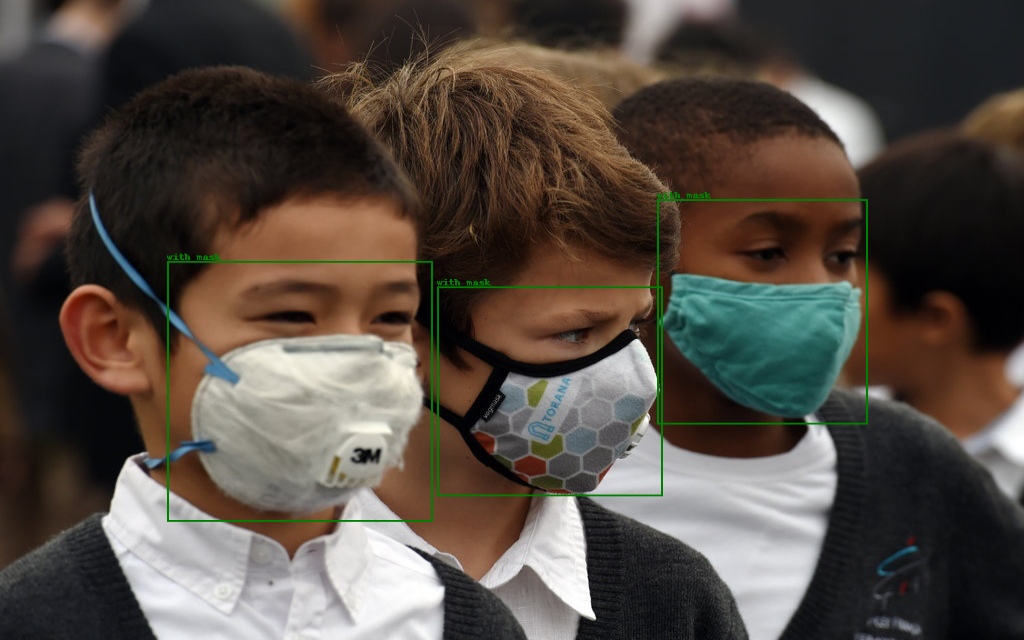
\includegraphics[width=\linewidth]{fig7a.png}\\
		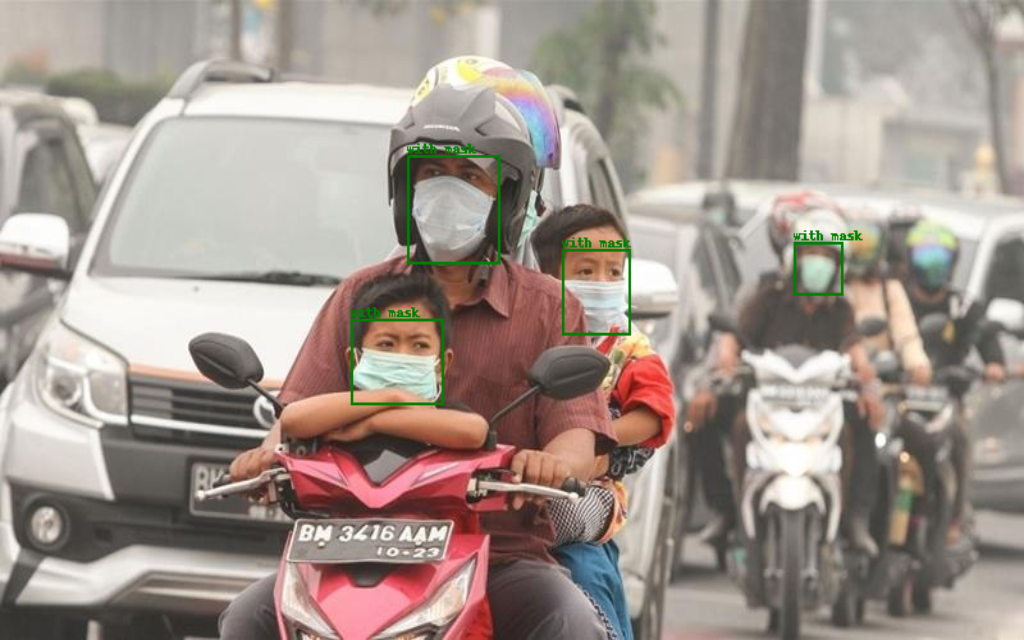
\includegraphics[width=\linewidth]{fig7e.png}
	\end{minipage}
	\begin{minipage}[t]{0.235\linewidth}
		\centering
		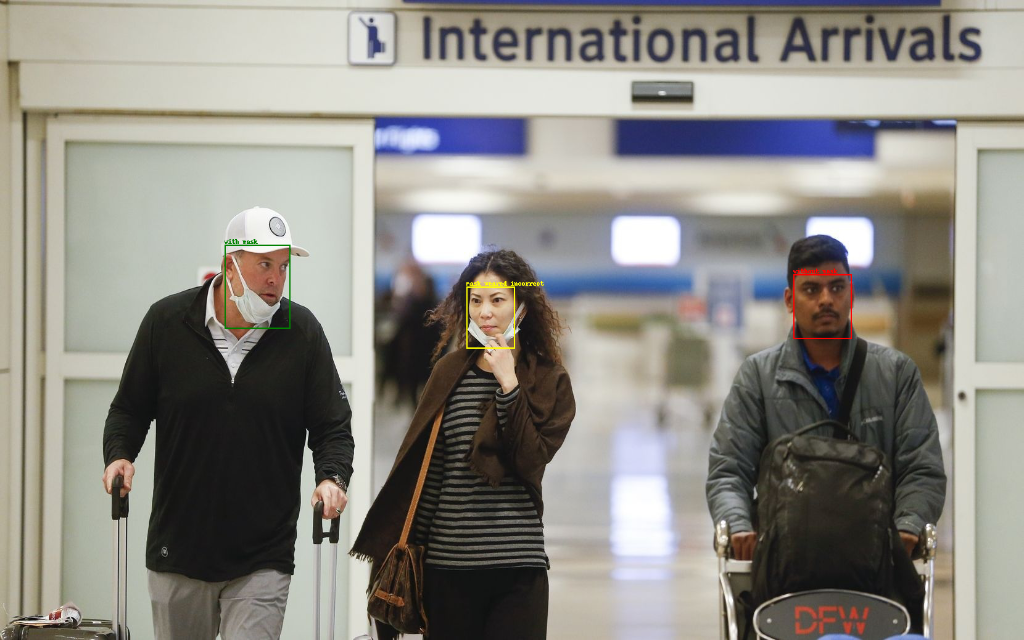
\includegraphics[width=\linewidth]{fig7b.png}\\
		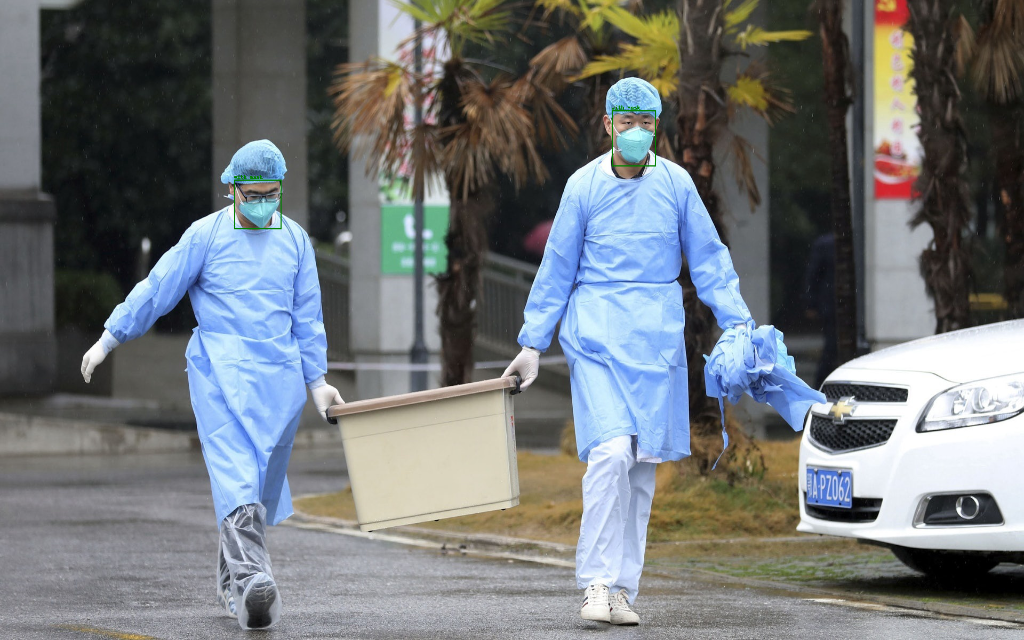
\includegraphics[width=\linewidth]{fig7f.png}
	\end{minipage}
	\begin{minipage}[t]{0.235\linewidth}
		\centering
		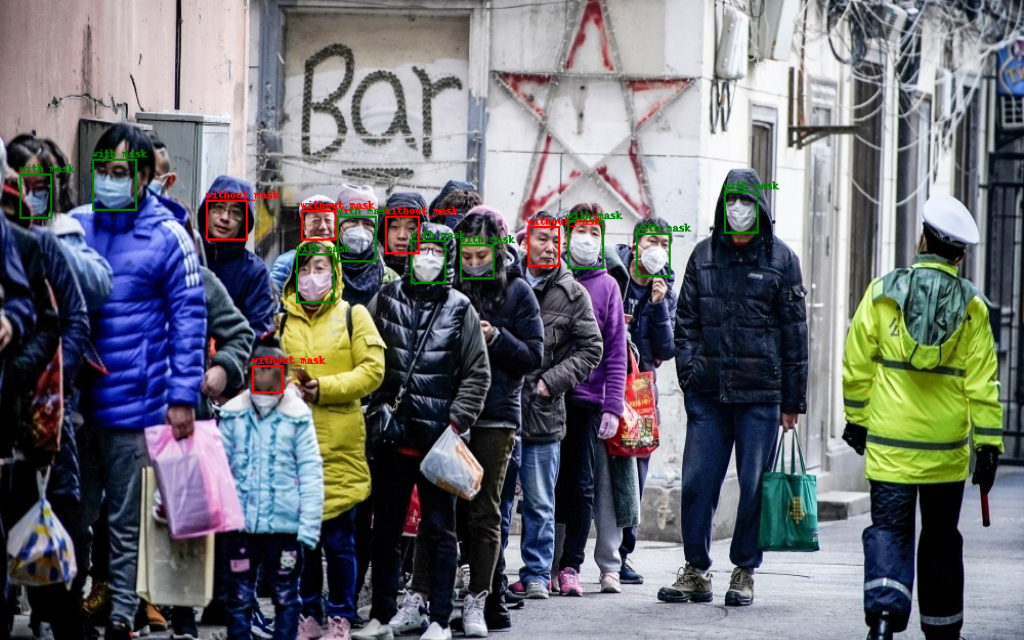
\includegraphics[width=\linewidth]{fig7c.png}\\
		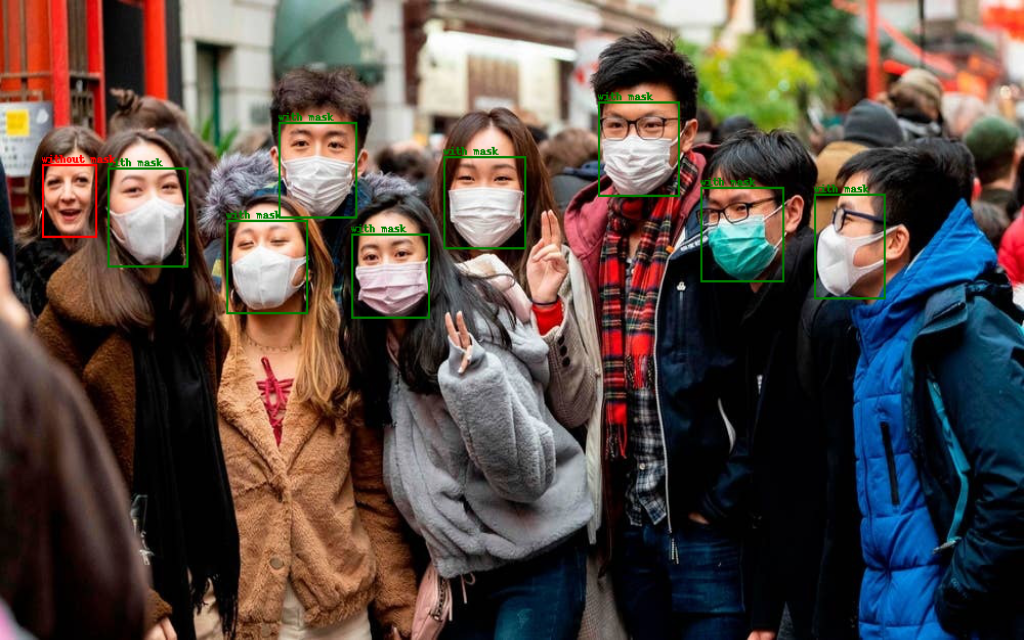
\includegraphics[width=\linewidth]{fig7g.png}
	\end{minipage}
	\begin{minipage}[t]{0.235\linewidth}
		\centering
		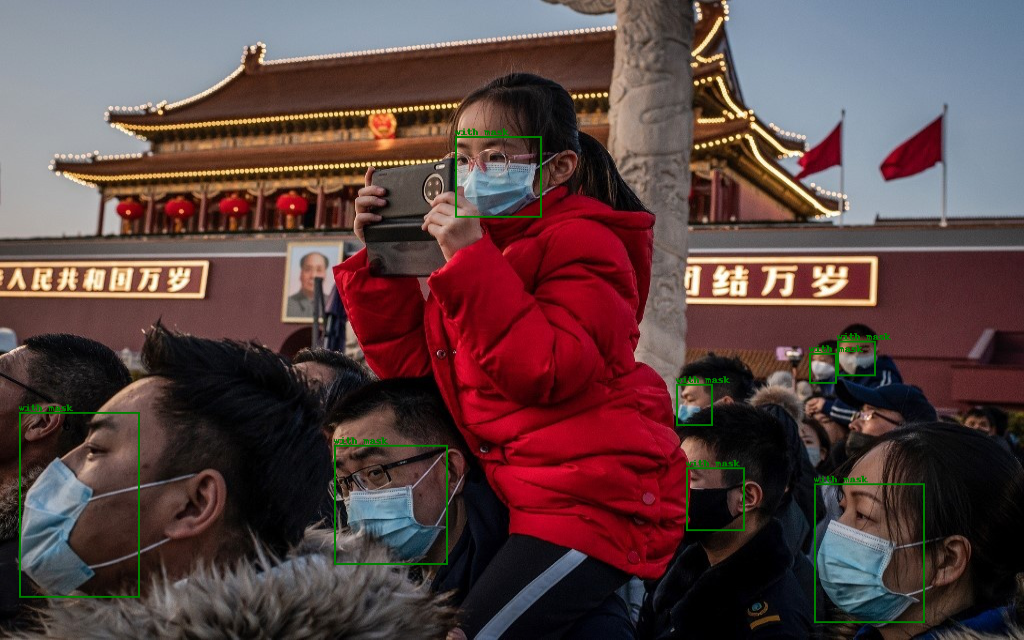
\includegraphics[width=\linewidth]{fig7d.png}\\
		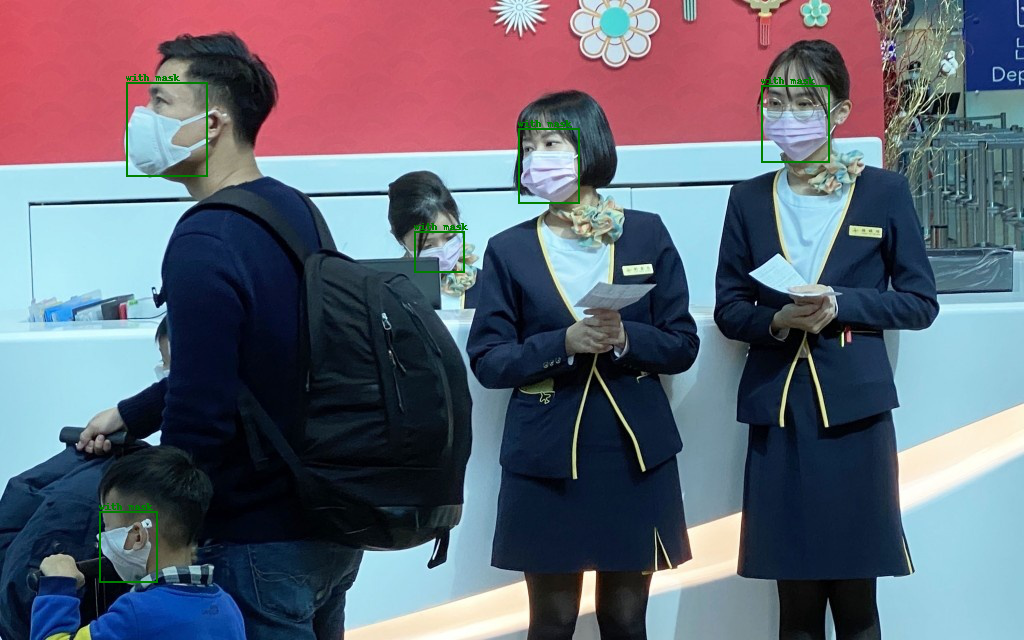
\includegraphics[width=\linewidth]{fig7h.png}
	\end{minipage}
	\caption{基于深度学习的口罩检测结果(部分)}
\label{fig:mask}
\end{figure}

\begin{table}[!ht]
	\centering
	\caption{基于深度学习的口罩检测评价指标}
	\begin{tabular}{c|c|cccc}
	\toprule
		&AP&AP$_{50}$&AP$_{75}$&AR$_1$&AR$_{10}$\\\hline
	Faster RCNN	&0.499&0.776&0.594&0.262&0.573\\
	\bottomrule
	\end{tabular}
	\label{tab:mask_metric}
\end{table}


实验在 PyTorch 提供的基于 COCO 数据集预训练的 Faster RCNN 模型调整预测器的输出类别后在 Mask Wearing 数据集上进行 finetune,训练 20--25 个 epoch 后验证集上的指标不在发生变化,在测试集上的评价指标如表 \ref{tab:mask_metric} 所示,检测结果如图 \ref{fig:mask} 所示。可以看到,深度学习模型可以对复杂场景进行较好的检测,如人群、侧脸或模糊的人脸,但同样由于样本邮箱,仍然会有检测失败的情形,如检测到不完整的人脸误判为未带口罩等。

\section{总结}
本文主要对与图像纹理相关的两个任务进行了探讨和实验,即纹理表征和纹理分割。相比较基于阈值的方法将图像分割为目标和背景两部分,基于聚类技术的纹理图像分割任务更加具有挑战性,其难点在于前期的纹理分析,如何较好地构建纹理特征,将在很大程度上对后续的纹理分割有影响。本文分别采用了灰度共生矩阵和 Gabor 滤波器两种方法分析图像的纹理特征。灰度共生矩阵方法简单,易于实现,但无法利用全局信息,与人类视觉模型不匹配,且计算复杂度较高,计算耗时。而 Gabor 滤波器具有较好的时-频局部话特性,其频率和方向与人类的视觉系统类似,特别适合于纹理表征与分割。


% Can use something like this to put references on a page
% by themselves when using endfloat and the captionsoff option.
\ifCLASSOPTIONcaptionsoff
  \newpage
\fi



%{\small
%\bibliographystyle{IEEEtran}
%\bibliography{reference/egbib}
%}

% that's all folks
\end{sloppypar}
\end{document}


